\section{Motivation}
\label{s:motivation}

% - characteristics of concurrency bugs
% - challenges / design requirements
% - limitations of existing approaches

This work is motivated by an observation that none of previous works
properly addresses characteristics of \textit{offending thread
  interleaving} (\ie, one that causes a concurrency bug).
%
As a consequence, previous works either \textbf{1)} suffer from
identifying whether interesting thread interleavings remain
untested~\cite{krace, conzzer, muzz}, or \textbf{2)} waste the
computing power by ineffectively exploring the search space of thread
interleaving~\cite{snowboard, razzer}.



In this section, we first comprehend why concurrency bugs manifest
depending on thread interleaving through a real-world concurrency bug
example.
%
We then define design goals for effectively discovering concurrency
bugs in the kernel, and summarize why existing approaches fall short
in satisfying the design goals.


\PP{Manifestation of concurrency bugs}
%
\begin{figure}[t]
  \centering
  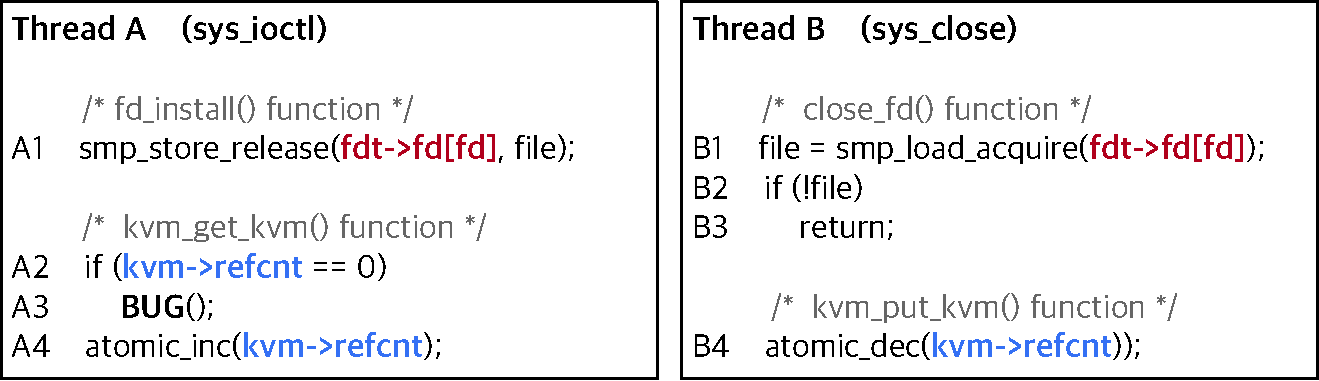
\includegraphics[width=0.9\linewidth]{fig/cve-2017-10661.pdf}
  \caption{Simplified code snippet of CVE-2017-17712. If \texttt{B1}
    is executed between \texttt{A2} and \texttt{A4}, concurrenct
    accesses on \texttt{inet->hdrincl} leads to uninitialized stack
    pointer usage on \texttt{rfv}, and an attacker may gain root
    privileges through a dedicated attack
    technique~\cite{stackspray}.}
  \label{fig:cve-2017-17712}
\end{figure}
%
In \autoref{fig:cve-2017-17712}, an uninitialized access bug may
manifest when two system calls are executed concurrently:
\texttt{sendmsg()} to send a message through an ipv4 socket, and
\texttt{setsockopt()} to modify an option of the ipv4 socket.

Let us assume \texttt{inet->hdrincl} is initially \texttt{1}.
%
During sending a message through the ipv4 socket, thread~A reads a
value of \texttt{inet->hdrincl} twice at \texttt{A2} and \texttt{A4}.
%
However, since these two read operations are not atomically executed,
thread~B may intervene in the middle of these two read operations.
%
In that case, if \texttt{B1} is executed between \texttt{A2} and
\texttt{A4}, thread~A reads different values of \texttt{inet->hdrincl}
at \texttt{A2} and \texttt{A4}, and dereference \texttt{rfv} without
initializing it.


\PP{Observation 1: Combined interleaving orders}
%
This example demonstrates that a concurrency bug is \textit{a combined
  result of a few interleaving orders}, where each interleaving order
denotes the execution order between an instruction pair that access
the same memory object.
%
In the example of \autoref{fig:cve-2017-17712}, two interleaving orders
are required to cause the uninitialized access bug.
%
First, \texttt{A2} should be executed before \texttt{B1} (\ie,
$\texttt{A2} \Rightarrow \texttt{B1}$\footnote{In this paper,
  $\texttt{X} \Rightarrow \texttt{Y}$ denotes that \texttt{X} is
  executed before \texttt{Y}}) to make thread~A not initialize
\texttt{rfv}.
%
Second, \texttt{B1} should be executed before \texttt{A4} (\ie,
$\texttt{B1} \Rightarrow \texttt{A4}$) to make thread~A dereference
uninitialized \texttt{rfv}.
%
Therefore, thread interleavings satisfying a combination of the two
interleaving orders (\ie,
$(\texttt{A2} \Rightarrow \texttt{B1}) \wedge (\texttt{B1} \Rightarrow
\texttt{A4}))$ cause the uninitialized access bug, while all other
thread interleavings do not.


\PP{Design goal 1: Informative interleaving coverage}
%
In order for a fuzzer to discover the uninitialized access bug, an
interleaving coverage should not be saturated until
$(\texttt{A2} \Rightarrow \texttt{B1}) \wedge (\texttt{B1} \Rightarrow
\texttt{A4}))$ is executed.
%
Otherwise, a fuzzer may think that there is no more interesting thread
interleaving in the multi-thread input, and stop searching for new
thread interleavings of the multi-thread input, missing the
uninitialized access bug.
%





\PP{Observation 2: Feedback from previous executions}
%
Interestingly, a previous execution that did not cause the
uninitialized access bug provides a feedback as to which thread
interleavings should be further explored.

To demonstrate this, let us assume we execute the two system calls in
\autoref{fig:cve-2017-17712} \textit{sequentially} such that the
execution of thread~A is followed by the execution of thread~B.
%
In this sequential execution, we can observe that three instructions,
\texttt{A2}, \texttt{A4}, and \texttt{B1} are executed in the order of
$\texttt{A2} \Rightarrow \texttt{A4} \Rightarrow \texttt{B1}$.
%
Unsuprisingly, we can easily imagine an interleaving of these three
instructions by flipping the execution order of \texttt{A4} and
\texttt{B1} (\ie,
$\texttt{A2} \Rightarrow \texttt{B1} \Rightarrow \texttt{A4}$).
%
And this imaginary interleaving is what exactly we are looking for; it
satisfies the combination of interleaving orders
$(\texttt{A2} \Rightarrow \texttt{B1}) \wedge (\texttt{B1} \Rightarrow
\texttt{A4}))$, and if we execute the imaginary interleaving, we can
discover the uninitialized access bug.

\PP{Design goal 2: Coverage-based interleaving search strategy}
%
In the perspective of fuzzing, previous executions are tracked using a
coverage metric.
%
Therefore, if an interleaving coverage metric tracks that
$\texttt{A2} \Rightarrow \texttt{A4} \Rightarrow \texttt{B1}$ is
\textit{explored} before, then a fuzzer can utilize interleaving
coverage to infer \textit{unexplored} thread interleavings (\eg,
$\texttt{A2} \Rightarrow \texttt{B1} \Rightarrow \texttt{A4}$), and
directly search for unexplored thread interleavings in future
iterations.
%
In this way, a fuzzer can quickly discover the uninitialized access
bug, without redundantly executing thread interleavings.



\subsection{Limitation of prior approaches}
\label{ss:existingapproaches}

\yj{Revise hint: Flow-OK, Clarification of text-Need work}
\begin{table}[t]
  \centering
  \resizebox{\linewidth}{!}{
  \begin{tabular}{l l l}
    \toprule
    & \thead{\textbf{Interleaving} \\ \textbf{coverage metric}} & \thead{\textbf{Interleaving} \\ \textbf{search strategy}} \\
    \midrule
    \textbf{Razzer~\cite{razzer}} & -- & Coverage-oblivious \\
    \textbf{Krace~\cite{krace}} & Alias coverage & Coverage-oblivious \\
    % & (single instruction pair) & \\
    \textbf{Conzzer~\cite{conzzer}} & Concurrent call pair & Coverage-based (limited) \\
    % & (single function pair) & (limited)\\
    \textbf{Snowboard~\cite{snowboard}} & -- & Coverage-oblivious \\
    \bottomrule
  \end{tabular}
}

%%% Local Variables:
%%% mode: latex
%%% TeX-master: "../p"
%%% End:

  \caption{Interleaving coverage metrics and interleaving search
    strategy of recent concurrency fuzzing. ``--'' indicates that a
    fuzzer does not adopt a concurrency coverage metric. \dr{TODO:
      rewording}}
  \label{table:motivation}
\end{table}

As shown in \autoref{table:motivation}, prior concurrency fuzzing
approaches adopt different interleaving coverage metrics and thread
scheduling control mechanisms.
%
Even though prior approaches achieve their own successes, we find that
their interleaving coverage metrics and thread scheduling control
mechanisms do not satisfy \textbf{Design goal 1} and \textbf{2}.


\PP{Less-informative interleaving coverage}
%
We find that previously proposed interleaving coverage metrics are
less-informative to determine whether a multi-thread input needs to be
further tested. Thus, they do not satisfy the \textbf{Design goal 1}.
%
This is because none of them consider a combination of interleaving
orders, which is a necessary condition for a concurrency bug to
manifest.
%
Specifically, alias coverage tracks individual interleaving orders,
and suffer from describing a combination of interleaving orders.
%
On the other hand, concurrenct call pair trakcs a pair of
concurrently-executed functions, and do not differentiate
interleavings taken place in the same function pair.




\begin{figure}[t]
  \centering
  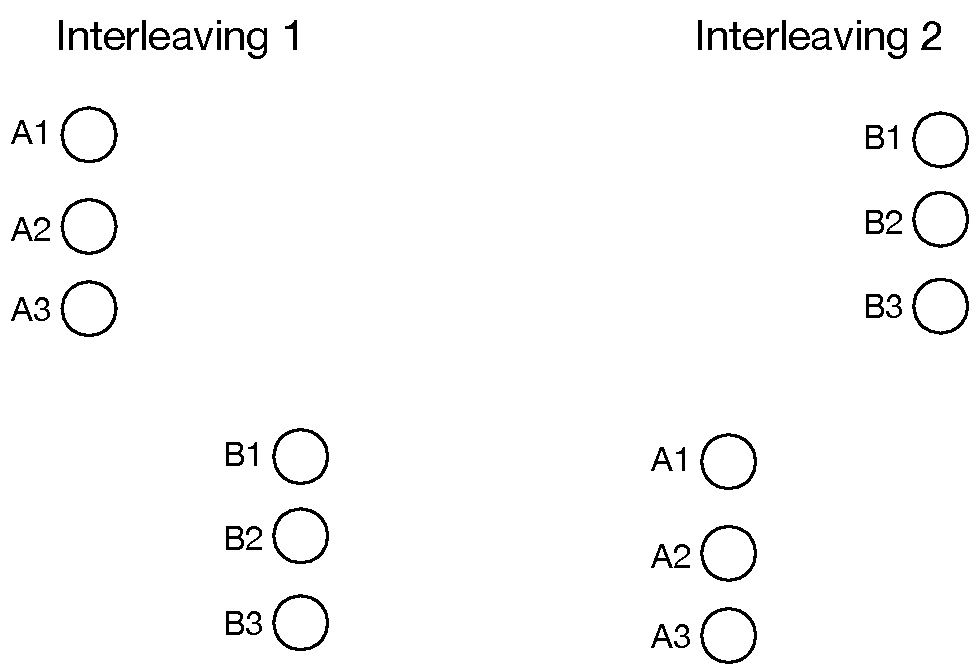
\includegraphics[width=0.90\linewidth]{fig/alias-coverage.pdf}
  \caption{Two thread interleavings between thread~A and thread~B
    described in \autoref{fig:cve-2017-17712}. The uninitialized
    access bug does not manifest in both interleavings.}
  \label{fig:alias-coverage}
\end{figure}


\autoref{fig:alias-coverage} shows two interleavings that saturate
existing interleaving coverage, where the uninitialized access bug
does not manifest.
%
In the two interleavings described in this figure, we can observe all
four individual interleaving orders regarding \texttt{inet->hdrincl}
(\ie, $\texttt{A2} \Rightarrow \texttt{B1}$ and
$\texttt{A4} \Rightarrow \texttt{B1}$ in Interleaving~\#1,
$\texttt{B1} \Rightarrow \texttt{A2}$, and
$\texttt{B1} \Rightarrow \texttt{A4}$ in Interleaving~\#2).
%
Therefore, alias coverage is saturated with these two thread
interleavings.
%
Moreover, concurrent call pair is also saturated with these two thread
interleavings, because once two functions, \texttt{sendmsg()} and
\texttt{setsockop()}, are executed concurrently, concurrnet call pair
does not matter how a thread interleaving occurs within the function
pair.

Therefore, they can possibly be saturated even before a concurrency
bug is exposed, misleading a fuzzer to de-prioritize a multi-thread
input in which a concurrency bug resides.




% \yj{This paragraph must be easy enough for reader to intuitively understand, but hard to digest discussions}
% However, they are not applicable to track behavioral changes\yj{what does it mean?} according
% to a combination of interleaving orders, mainly because they either
% track only a \textit{single} interleaving order~\cite{krace, muzz} or
% \textit{coarse-grained information} such as a pair of two
% concurrently-executed functions~\cite{conzzer}.
% \yj{I do not understand why tracking a single int. order and coarse-grain information are not able to track behavioral changes}

% Taking the example of KRace's alias coverage,
% \autoref{fig:alias-coverage} describes two thread interleavings that
% saturate alias coverage found between two system calls in
% \autoref{fig:cve-2017-17712}.
% %
% In these example interleaving scenarios, the uninitialized access does
% not manifest even after alias coverage is saturated, and a fuzzer may
% decide to stop searching for new thread interleavings in the two
% system calls.
% %
% While we do not enumerate all proposed interleaving coverage metrics
% here, we find that they all share the same limitation.


\PP{Coverage-oblivious interleaving search strategy}
%
Stemming from less-informative coverage metrics, proposed interleaving
search strategies are not properly directed by interleaving coverage,
and thus, do not satisfy the \textbf{Design goal 2}.

Since Razzer~\cite{razzer} and Snowboard~\cite{snowboard} do not make
use of interleaving coverage at all, they cannot rely on previous
executions in searching for unexplored thread interleavings.
%
Krace~\cite{krace} explores thread interleavings randomly without
considering what thread interleavings are explored before.

Whereas, Conzzer~\cite{conzzer} is the only work that attempts to
direct a fuzzer based on interleaving coverage.
%
However, its interleaving coverage (\ie, concurrent call pair) tracks
thread interleavings in the function-level granularity, and is limited
in distinguishing tested interleavings and untested interleavings in
the instruction-level granularity.
%
In other words, the Conzzer's interleaving search strategy can direct
a fuzzer to execute two functions, \texttt{raw_sendmsg()} and
\texttt{do_ip_setsockopt()}, concurrently.
%
But even after that, Conzzer suffers from triggering the uninitialized
bug since it is not aware of the execution order of instructions.


\dr{TODO: MUZZ}


%%% Local Variables:
%%% mode: latex
%%% TeX-master: "p"
%%% End:
